\documentclass[11pt]{article}
\usepackage{graphicx}
\usepackage{amssymb}
%\usepackage[nomarkers]{endfloat}
\usepackage{natbib}
\usepackage{setspace}
\usepackage{wasysym}
\usepackage{wrapfig}
\pagestyle{empty}
\textwidth = 7 in
\textheight = 9 in
\oddsidemargin = -0.5 in
\evensidemargin = -0.5 in
\topmargin = 0.0 in
\headheight = 0.0 in
\headsep = 0.0 in
\parskip = 0.1in
\parindent = 0in
\renewcommand{\Pr}{\mathbb{P}}
\usepackage{paralist}
\usepackage{url}
\newcommand{\href}[2]{\url{#2}}
\usepackage{tikz}
  \usetikzlibrary{shapes.geometric}
  \usetikzlibrary{arrows.meta,arrows}
  \usetikzlibrary{positioning,automata}
\tikzstyle{line}=[draw]
\usepackage{hyperref}
\hypersetup{backref,   linkcolor=blue, citecolor=red, colorlinks=true, hyperindex=true}
\begin{document}
\section*{Markov chains over a discrete state space acting in discrete time steps}

This document provides background and derivations for the demo at
    \url{http://phylo.bio.ku.edu/mephytis/disc-state-disc-time-Markov/index.html}
    \footnote{source code at \url{https://github.com/mtholder/mephytis}}.

The set of possible values that at stochastic process can visit is the ``state space'' of the model.
So a model of DNA evolution would have 4 states: $\mathcal{S} = \{A, C, G, T\}$.

A first order Markov process is one in which the probability distribution of the next state
    depends only on the current state -- not the previous history of the process.
Markov processes can be formulated as working on variables that have continuous or discrete state
    spaces.
They can also be formulated to work with a discrete or continuous index for moving from one state
    to the next step.
Often this indexing variable is thought of as time.
Here, we'll explore a discrete-state, discrete-time Markov chain.
Imagine that we have 4 states (I'll label them $A, C, G, T$), and the probability of switching
 states at each step is constant and equal no matter what the ``source'' state  or the
 ``destination'' state is.
When the states are DNA bases this model is called the
    \href{https://en.wikipedia.org/wiki/Models_of_DNA_evolution#JC69_model_(Jukes_and_Cantor_1969)}{Jukes Cantor 1969 model},
    and it is usually described in continuous time.
Here we'll imagine that we had some design (such as long-term experimental evolution study) that
    we can observe at even time intervals.
So we'll see time in steps.

We might want not know the probability of changing to a different state in one time step, so we
can use a parameter.
Let's call this parameter $s$.
If $x_i$ denotes the state of the process at time step $i$:
\begin{eqnarray*}
    \Pr(x_{i} \neq x_{i+1}) & = & s \\
    \Pr(x_{i+1} = C \mid x_{i}=A) & = & s/3 \\
    \Pr(x_{i+1} = G \mid x_{i}=A) & = & s/3 \\
    \Pr(x_{i+1} = T \mid x_{i}=A) & = & s/3 \\
    \Pr(x_{i+1} = A \mid x_{i}=A) & = & 1 - s
\end{eqnarray*}
and we could write similar formulas for the other starting states.
We can view the probability transition more compactly using the transition probability matrix
or graph:\\
\begin{figure}[h]
$\mathbf{P} = \left(\begin{array}{cccc} 1 - s & s/3 & s/3 & s/3 \\
 s/3 & 1 - s & s/3 & s/3 \\
 s/3 & s/3 & 1 - s & s/3 \\
 s/3 & s/3 & s/3 & 1 - s
 \end{array}\right)$
\hskip 3em
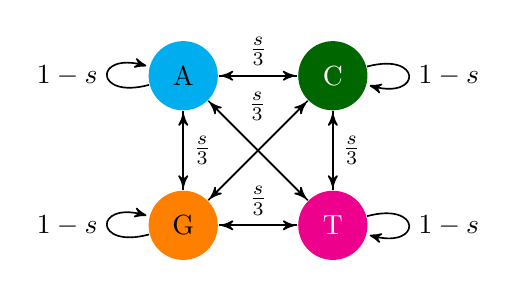
\begin{tikzpicture}[->,>=stealth',shorten >=1pt,auto,semithick,every state/.style={fill=red,draw=none,text=black,shape=ellipse}]
\node[state, fill=cyan] (A) {A};
\node[state, fill=black!60!green,text=white] (C) [right=of A] {C};
\node[state, fill=magenta,text=white] (T) [below=of C] {T};
\node[state, fill=orange,text=black] (G) [below=of A] {G};
\path (A) edge node {$\frac{s}{3}$} (C) ;
\path (A) edge node {$\frac{s}{3}$} (G) ;
\path (A) edge node [pos=.3] {$\frac{s}{3}$} (T) ;
\path (A) edge [loop left] node {$1-s$} (A) ;
\path (C) edge node {} (A) ;
\path (C) edge node {} (G) ;
\path (C) edge node {$\frac{s}{3}$} (T) ;
\path (C) edge [loop right] node {$1-s$} (C) ;
\path (G) edge node {} (A) ;
\path (G) edge node {} (C) ;
\path (G) edge node {$\frac{s}{3}$} (T) ;
\path (G) edge [loop left] node {$1-s$} (G) ;
\path (T) edge node {} (A) ;
\path (T) edge node {} (G) ;
\path (T) edge node {} (C) ;
\path (T) edge [loop right] node {$1-s$} (T) ;
\end{tikzpicture}
\end{figure}

There is no tendency to stay in one state longer than any other, so if you were to sample
    this process for a huge number of time steps (and $s>0$) then we'd expect to spend approximately
    equal time in each of the 4 states.
In the language of Markov chains, we'd say that the equilibrium frequency of each state is $1/4$
(or $\pi_A = \pi_C = \pi_G = \pi_T = 0.25$, in notation).

The probability rules above describe the transitions between adjacent steps of the chain,
    but we also need to know what state the process starts in.
It is common in molecular evolution to assume that the process has been running for a long time.
Thus it is reasonable to say that each of the 4 states are equally likely for the first state in
    the chain.

\subsection*{Inference}
Imagine that we have a sequence of observations at 10 evenly spaced time points for the state at a
particular site:\\
\begin{tabular}{ccccccccccc}
$i=$   & 0 & 1 & 2 & 3 & 4 & 5 & 6 & 7 & 8 & 9\\
$x_i=$ & $G$ & $G$ & $C$ & $C$ & $C$ & $C$ & $C$ & $C$ & $C$ & $A$
\end{tabular}
or (more compactly) $X=GGCCCCCCCA$.

{\bf Note}: we typically use the Jukes Cantor model when comparing sequence at the same site from
    different species -- here we are imagining that we saw the sequence as it was evolving in
    a series of steps down an unbranched  ancestor-descendant lineage. This is not the typical case!

How could we estimate what value of $s$ generated the sequence of observations?

We have a probabilistic model, so using a likelihood based procedure should be the most powerful
  approach (see
  \href{https://en.wikipedia.org/wiki/Likelihood_principle}{Wikipedia on the Likelihood Principle}).

So if our sample size is $n = 10$, we can write the likleihood as
\begin{eqnarray*}
\Pr(X\mid s) & = & \Pr(x_0)\prod_{i=1}^{n-1} \Pr(x_i \mid s, x_{i+1})\\
\end{eqnarray*}
Substituting $1/4$ for the start state, and $1-s$ for every time that state does not change and
$s/3$ for every time the base changes between adjacent states:
\begin{eqnarray*}
L(s) = \Pr(X=GGCCCCCCCA\mid s) & = & \left(\frac{1}{4}\right)(1-s)\left(\frac{s}{3}\right)(1-s)(1-s)(1-s)(1-s)(1-s)(1-s)\left(\frac{s}{3}\right)\\
 & = & \left(\frac{1}{4}\right)(1-s)^7\left(\frac{s}{3}\right)^2
\end{eqnarray*}

We could graph the likelihood as a funtion of $s$ and find the point that the maximizes the
likelihood.
Or we could use calculus to find the point where the likelihood profile is at it's maximum by
    finding the point where the derivative of the likelihood is 0.
It is easier to find the maximum on the log-likelihood scale:
\begin{eqnarray*}
\ln L(s) & = & \ln\left(\frac{1}{4}\right) + 7 \ln(1-s) + 2\ln\left(\frac{s}{3}\right)\\
& = & \ln\left(\frac{1}{4}\right) + 7 \ln(1-s) + 2\ln(s) - 2\ln({3})\\
\frac{d\ln L(s)}{d s} & = & \frac{-7}{1-s} + \frac{2}{s} \\
\end{eqnarray*}
We usually denote the maximum likelihood estimator of a parameter with a cute little hat, so
$\hat{s}$ is our MLE.
Because the likelihood is continuous the MLE will be the value of $s$ when the curve is flat (the
derivative is 0) or at one of the endpoints of the feasible range for $s$ ($s=0$ or $s=1$ in our
case because $s$ is a probability).
So, we find:
\begin{eqnarray*}
 \frac{-7}{1-\hat{s}} + \frac{2}{\hat{s}} & = & 0 \\
\frac{2}{\hat{s}} & = & \frac{7}{1-\hat{s}}
2 - 2\hat{s} & = & 7\hat{s} \\
\hat{s} & = & \frac{2}{9}\\
\end{eqnarray*}
Intuitively, the likelihood is maximized when $s$ is equal to the number of changes of state
    divided by the number of observations that could possibly have shown a change of state.
If we had put in a generic $n_d$ for the number of transitions where the states differed and
    $n_s$ for the number of transitions where the state stayed the same, we would have found
     that $\hat{s} & = & \frac{n_d}{n_s + n_d}$.

\end{document}